\chapter{Resultados}
\label{cap:04}

\section{Análise das Ferramentas Disponíveis no mercado}

%Lista e descreve brevemente ferramentas existentes (SonarQube, CodeClimate, PMD, ESLint, etc.).
Existem diversas ferramentas de mercado focadas na qualidade de código, embora muitas vezes com objetivos distintos da visualização educacional de grafos.

Sendo assim, esta seção busca apresentar algumas das principais ferramentas disponíveis no mercado, com o objetivo de analisar suas funcionalidades para embasar a construção da ferramenta proposta nesta pesquisa.

\subsection{SonarQube}

A ferramenta SonarQube (Figura \ref{fig:sonarqube_screen}) é uma plataforma de código aberto (\textit{open source}) voltada à inspeção contínua da qualidade do código. Em vez de apenas gerar listas de erros, a ferramenta permite a análise, o rastreamento e o gerenciamento da qualidade do software de modo proativo ao longo do tempo \citeonline{sonarqube}.
\begin{figure}[H]
    \centering
    \caption{Captura de tela da interface do SonarQube}
    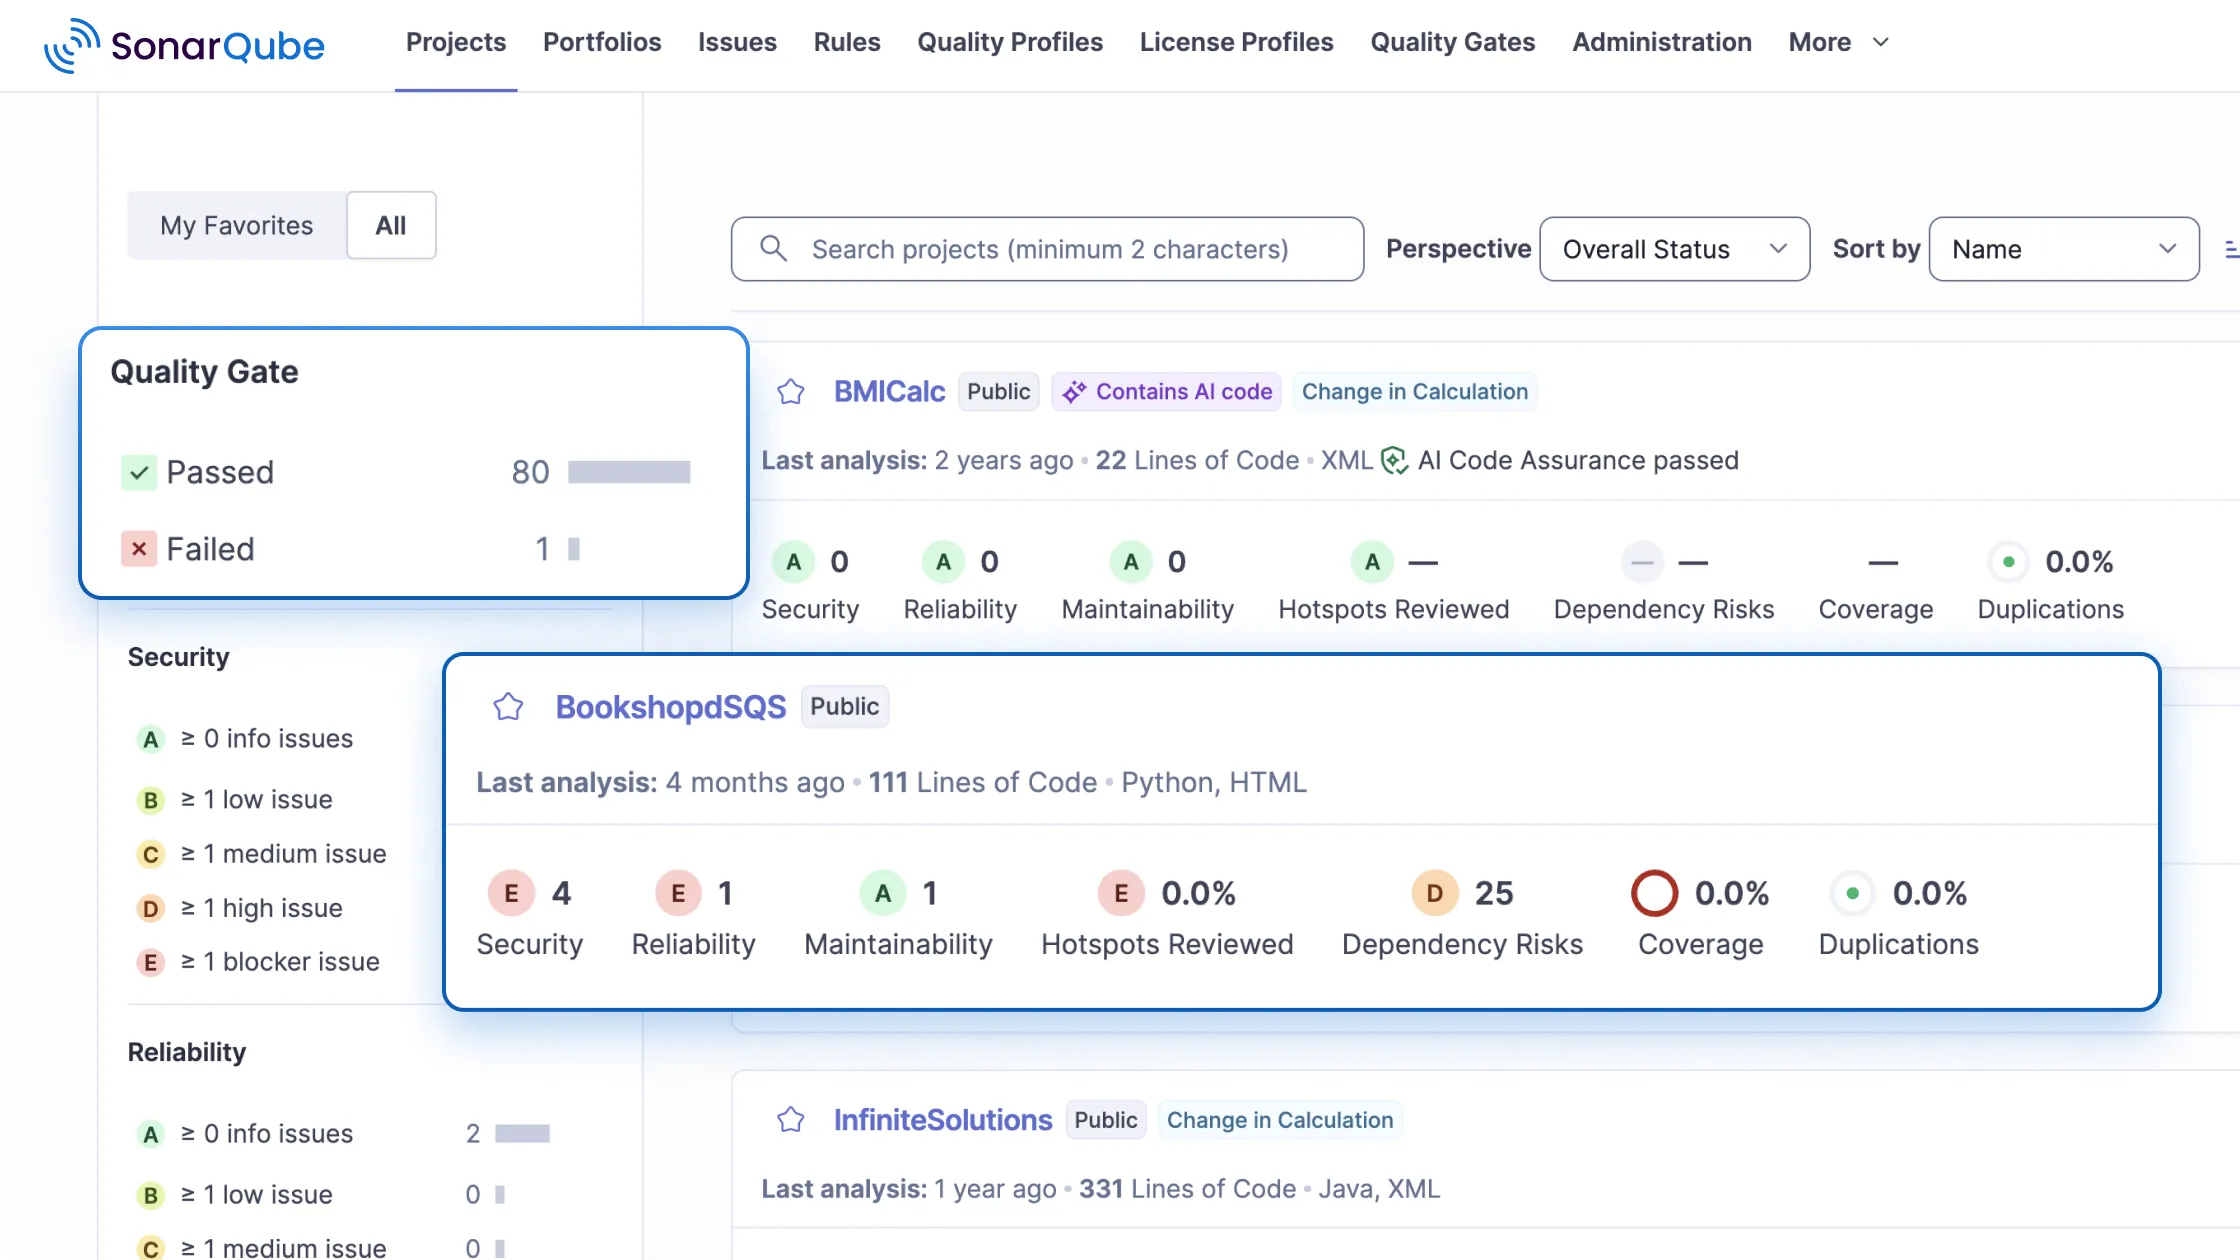
\includegraphics[width=0.75\linewidth]{imagens/sonarqube-screen.png}
    \fonte{Adaptado de SonarSource (2026).}
    \label{fig:sonarqube_screen}
\end{figure}



A plataforma atua na exibição de potenciais \textit{bugs}, violações de convenções e boas práticas, além de medir cobertura de testes, duplicação de código e complexidade ciclomática. Dessa forma, possibilita a inspeção contínua por meio de \textit{dashboards} e histórico de análises, integrando-se às principais IDEs do mercado \citeonline{campbell2013sonarqube}.

No entanto, embora a plataforma possua uma versão gratuita, algumas funcionalidades avançadas e recursos gerenciais são comerciais e requerem pagamento. Ademais, a ferramenta está sujeita à ocorrência de falsos positivos e exige configuração adequada para o contexto de cada projeto. Vale ressaltar que, apesar de calcular a complexidade ciclomática, os dados são exibidos principalmente em painéis e relatórios, sem focar na visualização gráfica e interativa do Grafo de Fluxo de Controle (GFC) do algoritmo.


\subsection{Codacy}

O Codacy (Figura \ref{fig:codacy_dashboard}) é uma plataforma de análise estática, gratuita para projetos de código aberto, com foco na melhoria da qualidade do software, no aumento da cobertura de testes e na prevenção de falhas de segurança \citeonline{ardito2020tool}. Distanciando-se de métricas matemáticas puras, a ferramenta prioriza uma abordagem prática na identificação de \textit{bugs} e comportamentos indefinidos em uma ampla variedade de linguagens de programação \citeonline{ardito2020tool}.

\begin{figure}[h]
    \centering
    \caption{Interface do Dashboard de Monitoramento Codacy}
    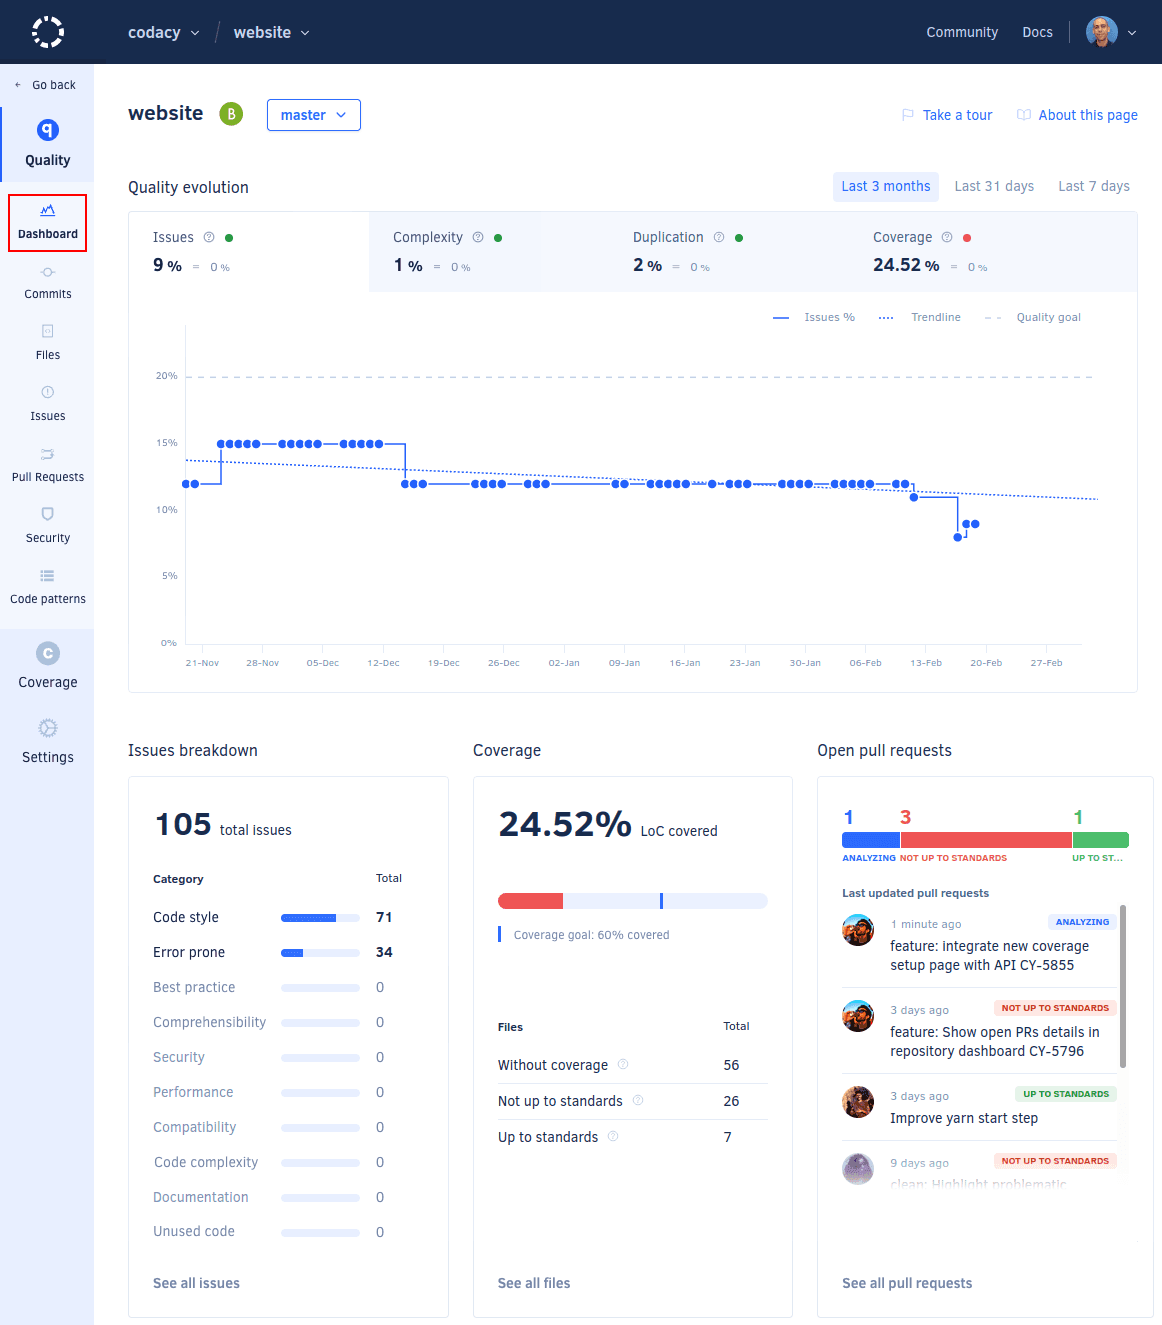
\includegraphics[width=0.5\linewidth]{imagens/codacy-fromCodacyDocs-print.png}
    \label{fig:codacy_dashboard}
    \fonte{Documentação Oficial do Codacy (2026). }
\end{figure}

Esta plataforma destaca-se pela sua interface amigável e pela facilidade de configuração e integração aos projetos \citeonline{imbugwa2021case, rahmawati2023analisis}. Como diferencial, o Codacy consolida estatísticas sobre propensão a erros, estilo e segurança em um \textit{dashboard}, atribuindo uma nota geral ao projeto que varia de "A" (alta qualidade) a "F" (baixa qualidade) \citeonline{ardito2020tool, imbugwa2021case}.

No entanto, a ferramenta apresenta limitações quanto à transparência da agregação de métricas para a nota final, o que pode dificultar a compreensão do peso de cada fator avaliado \citeonline{ardito2020tool, imbugwa2021case}. A análise depende frequentemente de \textit{linters} de terceiros e pode gerar falsos positivos \citeonline{imbugwa2021case}. Consequentemente, embora avalie categorias de complexidade \citeonline{ardito2020tool}, seus resultados permanecem restritos a notas agregadas e painéis, mantendo a lacuna analítica de não fornecer uma representação gráfica clara do fluxo lógico do algoritmo analisado.

\subsection{ESLint}

O ESLint (Figura \ref{fig:eslint_playground_demo}) é um \textit{linter} plugável e uma ferramenta de análise estática amplamente utilizada, projetada para JavaScript e extensível ao TypeScript por meio de \textit{plugins} \citeonline{eslint, tomasdottir2020adoption, bhutani2024analysing}. Sua função principal é examinar o código sem executá-lo, utilizando sua representação sintática para identificar padrões, impor convenções de estilo e sinalizar erros, ajudando a manter a consistência do projeto \citeonline{tomasdottir2017why}. A ferramenta destaca-se por sua flexibilidade, permitindo a adoção de regras e \textit{presets} da comunidade \citeonline{tomasdottir2020adoption}.

\begin{figure}[H]
    \centering
    \caption{Playground do ESLint exibindo a identificação de erros de sintaxe e estilo.}
    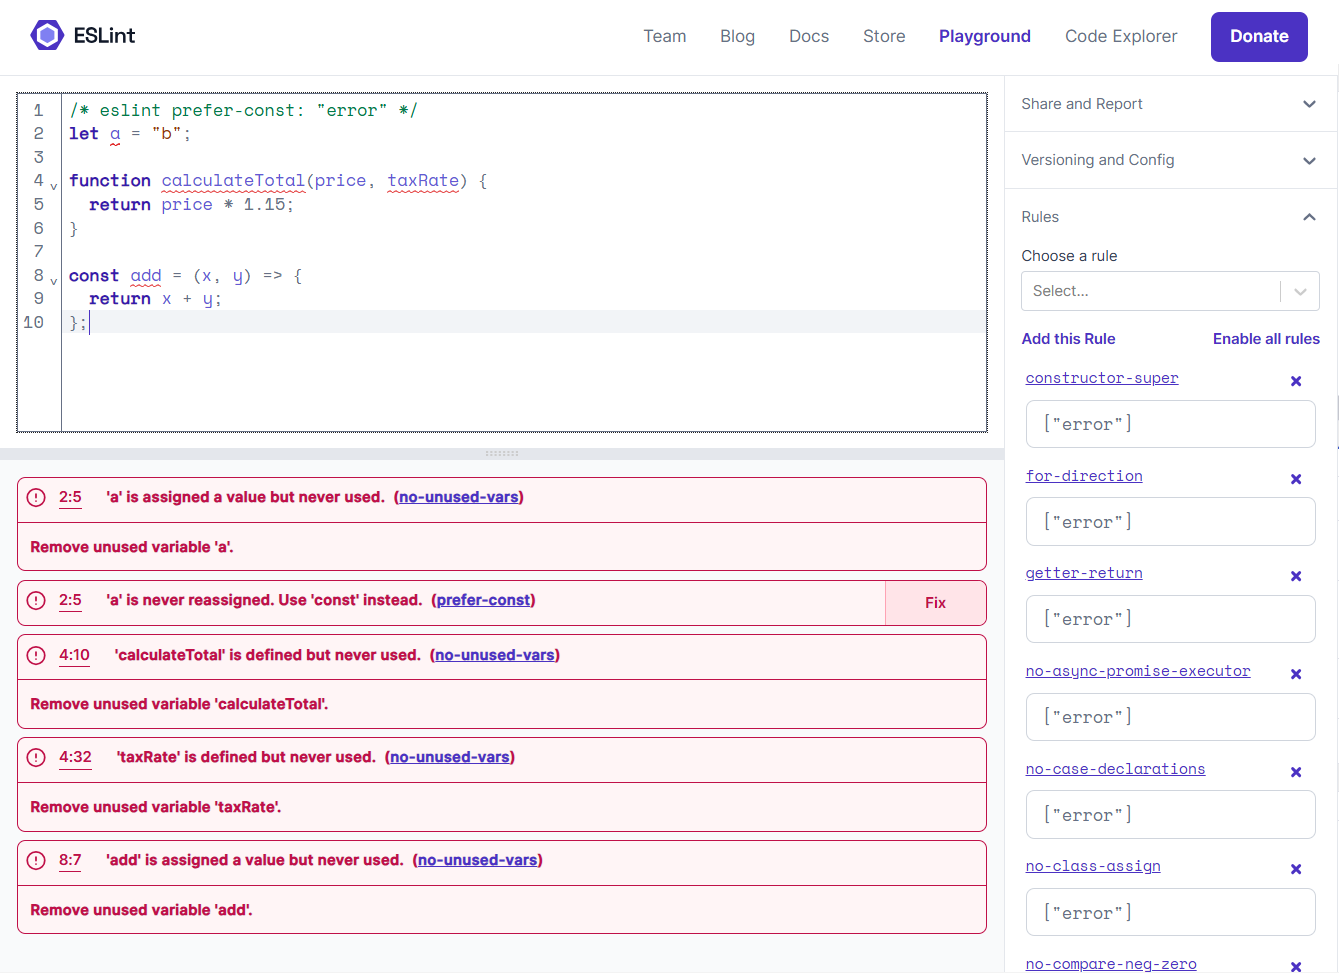
\includegraphics[width=0.75\linewidth]{imagens/eslint-capture.png}
    \fonte{Adaptado de ESLint (2026).}
    \label{fig:eslint_playground_demo}
\end{figure}

Além de oferecer correção automática (auto-fix) e um ecossistema extensível \citeonline{rafnsson2020fixing, bhutani2024analysing}, o ESLint possui fácil integração com IDEs e pipelines de CI/CD, fornecendo \textit{feedback} em tempo real e atuando como um recurso educacional para os desenvolvedores \citeonline{bhutani2024analysing, murugaraj_automated, tomasdottir2017why}.

Apesar dessas vantagens, a ferramenta possui limitações técnicas. A avaliação do ESLint é orientada principalmente à análise estática de arquivos e regras configuradas no projeto, o que limita a identificação de problemas que dependem de interações complexas entre módulos, execução real ou dependências externas \citeonline{rafnsson2020fixing}. Sua eficácia também esbarra na natureza dinâmica do JavaScript, não sendo capaz de prever todos os erros em tempo de execução \citeonline{tomasdottir2017why, bhutani2024analysing}. Além disso, a complexidade de configuração e a ausência de provas formais de correção podem gerar falsos positivos; esse excesso de avisos frequentemente resulta em uma ``fadiga de alertas'', levando os desenvolvedores a ignorarem os reportes ou a perderem a confiança na análise \citeonline{tomasdottir2020adoption, rafnsson2020fixing, pfeiffer2022technical}.

No que diz respeito à análise da estrutura lógica, essa restrição torna-se relevante para o escopo desta pesquisa. Embora possua regras para alertar quando a complexidade ciclomática de uma função excede um limite pré-estabelecido, o ESLint não tem como foco apresentar uma visualização interativa do fluxo de execução do algoritmo \citeonline{eslint}. Consequentemente, a ferramenta restringe a compreensão estrutural a alertas e diagnósticos textuais, sem prover uma visualização gráfica do fluxo de controle.


\section{Levantamento de Requisitos da Ferramenta Guy}

Esta seção apresenta um levantamento de requisitos inicial da ferramenta Guy, proposta nesta pesquisa.

O acesso à ferramenta será realizado diretamente no ambiente de desenvolvimento por meio de uma extensão para o editor \textit{Visual Studio Code} \citeonline{microsoft_vscode}. Um requisito fundamental é que a análise estática seja executada de forma estritamente local. Isso será possível graças ao uso de tecnologias como o \textit{WebAssembly} e o Tree-sitter, que atuarão na construção eficiente da árvore sintática, podendo integrar-se ao ecossistema do ESLint para potencializar o fornecimento de diagnósticos.

Essa arquitetura garante que o processamento léxico e sintático do código ocorra de forma estritamente local, diretamente no ambiente de desenvolvimento do usuário. Dessa forma, assegura-se um \textit{feedback} em tempo real durante a escrita do código. Além disso, essa abordagem favorece a conformidade (\textit{compliance}) com políticas de segurança corporativa e privacidade, ao proteger a propriedade intelectual e evitar a exposição do código a ambientes de terceiros, eliminando os custos com infraestrutura de nuvem, uma vez que dispensa o envio dos trechos desenvolvidos para servidores externos.

No aspecto funcional, a principal entrega do sistema consiste na renderização visual interativa do Grafo de Fluxo de Controle (GFC) assim que o código-fonte é analisado. A interface deverá permitir que o programador interaja com o grafo gerado, correlacionando visualmente os nós de decisão e as arestas direcionadas com as respectivas linhas do arquivo aberto no editor. Em conjunto com essa visualização, a extensão tem o requisito de calcular e exibir a métrica de Complexidade Ciclomática, atuando como um indicador sobre a complexidade lógica e a testabilidade do código.

Para apoiar o desenvolvedor na análise da qualidade estrutural do software, a extensão servirá como uma ferramenta visual para a identificação dos caminhos linearmente independentes no grafo. O sistema fornecerá os dados estruturais necessários para que o programador elabore casos de teste alinhados aos fluxos identificados. Dessa forma, a análise estática converte-se em uma etapa de apoio prático ao diagnóstico e à compreensão da lógica do código.

\section{Prototipagem e Design da Ferramenta Guy}

O usuário aciona a extensão com o editor de código aberto e em foco. Em resposta, a ferramenta abre uma janela lateral, de forma semelhante a uma pré-visualização de Markdown, apresentando o Grafo de Fluxo de Controle (GFC) e o cálculo da Complexidade Ciclomática, representada por \(V(g)\).
A partir dessa visualização, o usuário pode selecionar vértices e arestas do grafo para navegar diretamente até os trechos correspondentes do código-fonte, estabelecendo uma relação interativa entre a representação visual e a implementação analisada.

Essa proposta atende aos principais requisitos definidos para a ferramenta: execução local, sem envio do código-fonte para servidores externos; apresentação do GFC em conjunto com o valor de \(V(g)\); e interação direta entre os elementos do grafo e as regiões correspondentes do código.

% --- Diagramas mermaid ---
% Os diagramas originais estão nos ficheiros:
% - diagrama_casos_uso_guy.mmd
% - diagrama_cenarios_guy.mmd
%
% Os arquivos SVG gerados pelo processo de CI estão incluídos no repositório e podem ser inseridos diretamente nas figuras abaixo.

\begin{figure}[H]
  \centering
    \caption{Diagrama de casos de uso da Ferramenta Guy.}
  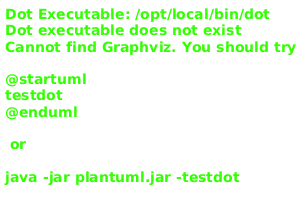
\includegraphics[width=1\linewidth]{imagens/diagrams/diagrama_casos_uso_guy.png}
  \fonte{Elaborada pelo autor}
  \label{fig:casos_uso_guy}
\end{figure}

\begin{figure}[H]
  \centering
    \caption{Diagrama de cenários (sequência) da Ferramenta Guy.}
  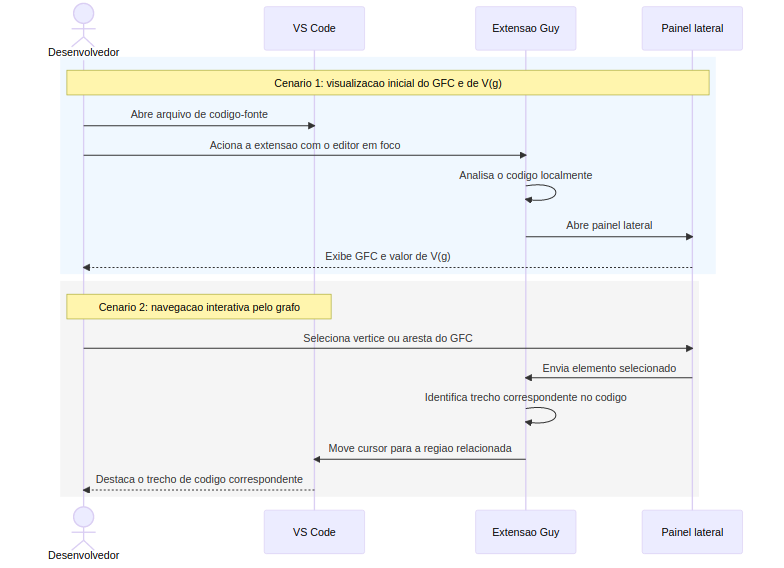
\includegraphics[width=1\linewidth]{imagens/diagrams/diagrama_cenarios_guy.png}
  \fonte{Elaborada pelo autor}
  \label{fig:cenarios_guy}
\end{figure}

% Fim das instruções para diagramas

\section{Implementação da Ferramenta Guy}
%desenvolvimento e configuracao no VSCode - pode criar subsecoes

%explicar com trechos de codigo

%adicionar o link do github com o codigo compelto

\section{Validação da Ferramenta Guy}

\subsection{Experimento I: Código com Looping e Ifs}

% explicar o objetivo do experimento - o que tem no codigo a ser gerado o GFC

% colocar um print do codigo

% colocar o print do GFC gerado no VSCode

% apresentar as metricas

\subsection{Experimento II: XXX}

\subsection{Experimento III: XXX}

\section{Análise Qualitativa da Ferramenta Guy}

% Pontos Positivos e Pontos Negativos (Pontos de Melhorias / Limitações)
